\section {Method and material}

\begin{figure}[t]
	\begin{centering}
		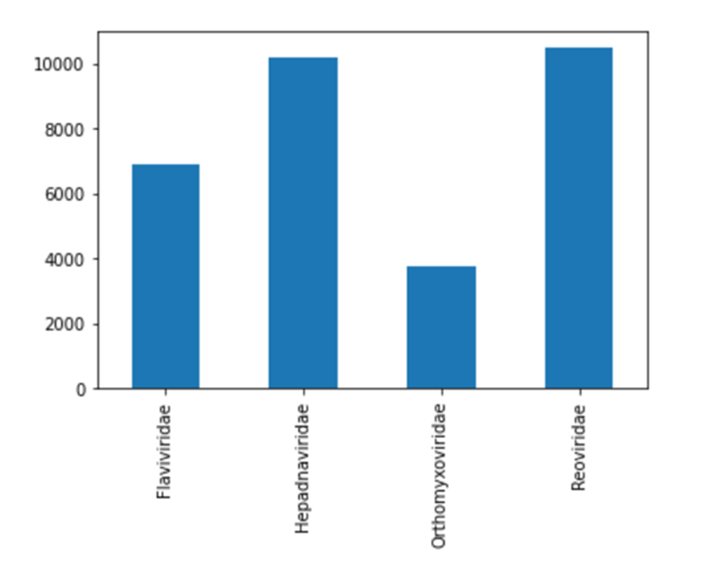
\includegraphics[width=.48\textwidth]{Figures/dist.png}
	\caption{distribution  }
\label{fig:distr}
\end{centering}
\end{figure}

\subsection{Data set}
\label{sec:obj:det}


In this research we used sequences of Vertebrate viruses obtained from Virosaurus database in FASTA format. Virosaurus contains full-length genomes (monopartite genomes) or segments (segmented genomes) for all virus families comprising at least one species infecting vertebrates.  Virosaurus also provides complete virus sequence dataset for all those viruses, which comprises complete genomes for non-segmented viruses, and complete segments for segmented viruses. The FASTA headers have been annotated with metadata, such as the viral nucleic acid (RNA, DNA, or RNA/DNA), and other information like the virus species, hosts, virus family, taxonomy identifier, and the official acronym name of the species.  The header contains 11 different topics annotated by a controlled vocabulary. Data comes from GenBank, ICTV, ViralZone and manual curation. 
FASTA header: 
\begin{lstlisting} 
<GenbankID> :<SequenceID> ; usual name=<common clinical name>;clinical 	level=<SPECIES or GENUS>; clinical typing=<unknown or subtype name>; 	species=<species name>;taxid=<NCBI taxID>;   acronym=<virus acronym>; nucleic 	acid=<DNA, RNA or DNA/RNA>; circular=<Y or N>; segment=<N/A or segment name>;
\end{lstlisting}
where, 
\begin{itemize}
\item{GenbankID}  Genbank accession number. 
\item{SequenceID} the Sequence ID is a unique identifier like GENE\_583-3988. 
\item{Usual name} Name of clinical level entity 
\item{Clinical level} Gives the taxonomic level suggested to be relevant for usual clinical diagnostics. 
\item{Clinical typing} Unknown by default. Otherwise contains data clinically relevant below species level. 
\item{Species} indicates the current official species name, as reported by International Committee on Taxonomy of viruses (ICTV, 07\_19). 
\item{Taxid} Taxonomy identifier from NCBI taxonomy database: 
Acronym=Official acronym name of the species 
\item{Nucleic acid} Nature of viral genome, either RNA or DNA, or RNA/DNA for retro-transcribing viruses (Ortevirales). 
\item{Circular}Y or N for yes or no. This is essential for to map efficiently reads at both extremities of the FASTA sequence. 
\item{Segment} N/A for monopartite viruses. For segmented genomes: official segment name as reported in ViralZone database
\end{itemize}
 
As the dataset is large and some species are new and some species are unknown, we have trained our model on the prediction of four family viruses which are Flaviviridae,  Hepadnaviridae, Orthomyxoviridae and Reoviridae. Of those four virus families we have chosen some virus species to be able to predict the specific species name of a given virus or predict what a new virus is close to from the data we have.

\begin{itemize}
\item{Flaviviridae}: Flaviviridae is a family of viruses that includes several human pathogens, such as, dengue, West Nile, and yellow fever viruses. These viruses are single stranded RNA viruses that are transmitted to humans by arthropod vectors, such as mosquitoes. The Flaviviridae family is divided into three genera: Flavivirus, Pestivirus, and Hepacivirus. The flavivirus genus  contains more than 70 distinct viral species.  

\item{Hepadnaviridae}: Hepadnaviridae is a family of viruses that includes the hepatitis B virus (HBV). HBV is a small, partially double-stranded DNA virus that causes acute and chronic liver infections in humans. 

\item{Orthomyxoviridae}: Orthomyxoviridae is a family of viruses that includes several human pathogens, such as influenza A, B, and C viruses. These viruses are responsible for causing seasonal influenza. The influenza viruses are negative-sense, single-stranded RNA viruses. They have a segmented genome, which means that the viral genome is composed of multiple pieces of RNA.

\item{Reoviridae}: Reoviridae is a family of viruses that includes several pathogens, such as rotaviruses, which are responsible for causing severe diarrhea in infants and young children, and orbiviruses, which are responsible for causing several diseases in animals.  The Reoviridae have several species: African horse sickness virus, bluetongue virus, etc 
\end{itemize}

The distribution of these families in the data set is shown in Figure 1.

\subsection{K-mers Sequencing}










